\documentclass{article}
\usepackage[hybrid]{markdown}
\usepackage{lineno}
\linespread{2} 
\linenumbers
\usepackage{natbib}
\usepackage{amsmath}
\usepackage{algorithm}
\usepackage{algpseudocode}
\bibliographystyle{abbrvnat}
\setcitestyle{
    authoryear,
    open={(},
    close={)}
}
\usepackage{hyperref}
\hypersetup{
    urlcolor=blue,
    colorlinks=true,
    linkcolor=black
}
\usepackage{geometry}

 \geometry{
     a4paper,
     left=25mm,
     right=25mm,
 }
 \title{Clockor2:  Inferring global and local strict molecular clocks using root-to-tip regression}

\begin{document}
\maketitle
\begin{centering}
Leo A. Featherstone$^{\ast,1}$, Sebastian Duchene$^1$, Wytamma Wirth$^{1}$\\
$^{1}$ Peter Doherty Institute for Infection and Immunity, University of Melbourne, Australia.\\
*email: leo.featherstone@unimelb.edu.au
\end{centering}

\section*{Abstract}


\section*{Introduction}
- Need to give distrinction of strict, global and local molecular clocks.
- RTT is still an attractive method for calibrating string molecular clocks due to its simplicity. However, as phylodynamics grows to consider larger datasets, and an increasing diversity of non-viral pathogens, strict molecular clocks with a global rate becomes an increasingly restrictive assumption. To this end we introduce clockor2, a root-to-tip regression tool that  can infer local as well as global string molecular clocks.
- Need to include specific examples of where local clocks emerge: VOCS, bacteria, host - mink
- Data also getting larger - think hill, du plessis, nordic? (will surely be many others)

- Mention usual way of fitting local clocks - beast and how many hours it can expect to take

\section*{Methods}
\subsection*{Dependencies}
Clockor2 has three key dependencies for handling, and plotting trees and RTT data. Trees are handled and manipulated using the phylotree.js library \citep{shank_phylotreejs_2018}. Phylocanvas is used to viaualise trees and plotly.js is used to plot RTT data \citep{abudahab_phylocanvasgl_2021}.

\subsection*{General model for global and local strict clocks}
\begin{figure}[H]
\centering
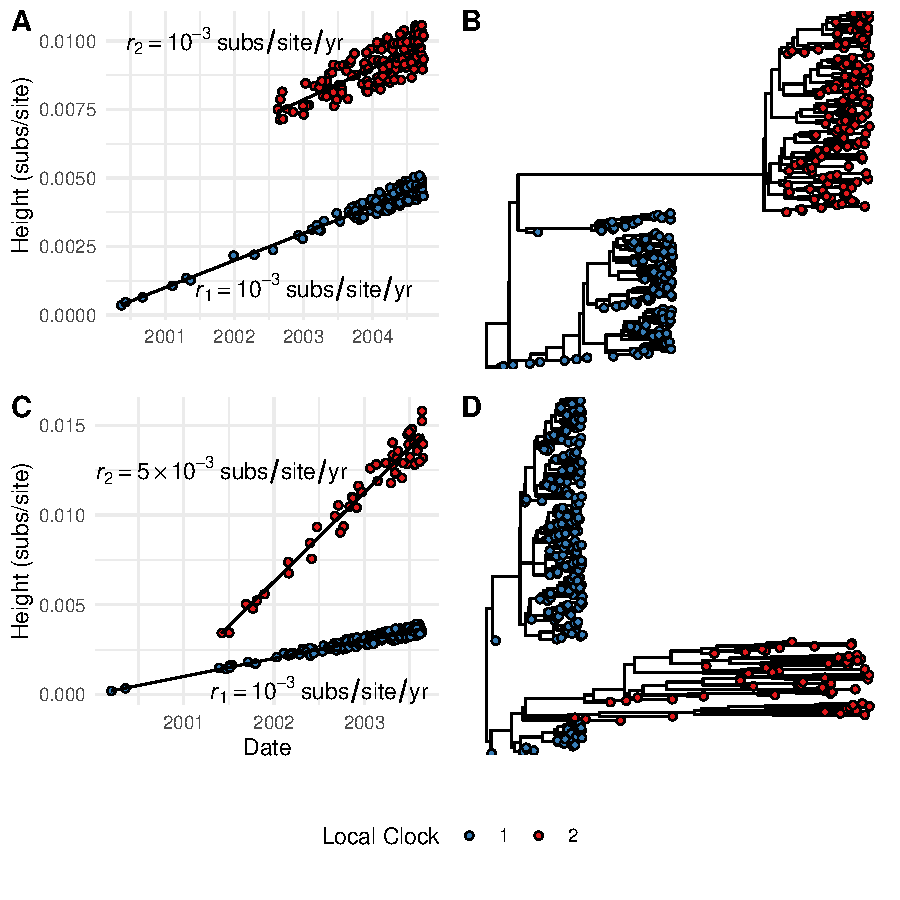
\includegraphics[1\linewidth]{figures/egRTT}
\caption{Example RTT}
\label{fig:egRTT}
\end{figure}

Root to tip regression models strict evolutionary rates as the slope of a linear regression between tip heights and their sampling dates. If we denote the evolutionary rate as $r$ (usually in units of $subs/site/time$), tip heights as $h$ (usually in units of $subs/site$), $o$ as the intercept (interpreted as origin), and sampling times as $t$, then the model is:
\begin{equation*}
    h = rt + o + \epsilon
\end{equation*}
where epsilon is the error term.

Clockor2 uses a generalisation of this model to accommodate local clocks. For a given tree with a set of tips $T$, we define local clocks as pertaining to \textit{groups} of tips $g_i$ and a rate parameter for each ($r_i$). For a strict clock model with two local clocks, we then write:
\begin{equation*}
    h = 
    \begin{cases}$
    $r_{1}t + o + \epsilon, \textnormal{ if tip }\in g_1$\\
    $r_{2}t + o + \epsilon, \textnormal{ if tip }\in g_2$
    $
    \end{cases}
\end{equation*}

We refer to groups instead of clades because a while a collections of tips belonging to one local clock are necessarily monophyletic, they do not necessarily comprise a clade. This occurs when two or more local clocks are nested. The tips comprising the outer clock(s) cannot comprise a whole clade if another local clock is nested within it. Below we give an example of a local clock model with two clocks. TODO - add figure.

Using the assumption of independent samples, we can then write the likelihood of the model by factorising the likelihood of the overall model. TODO: See supps for derivation.

$R^2$ values for each clock are then an indication of clock-like behaviour with a value of one indicating exact evolution according to a strict clock. 

TODO: Point about statistical non-independence of samples

\subsection*{Algorithm for local clock search}
Where it is hypothesised that a datasset contains local clocks, clockor2 provides functionality to corroborate this hypothesis by performing a search for local clocks in the tree. Briefly, the algorithm takes a maximum number of clocks and a minimum group size for each local clock as input parameters. It then iterates through all combinations of internal nodes from which local clocks can descend to induce  configuration of local clocks satisfying the maximum number of local clocks and minimum group size. Importantly, the clock search algorithm test for a number of clocks up to an including the maximum number so that more parsimonious configurations with fewer clocks may be found. Configurations are compared using the information criteria outlined above. Again, we reccommend the BIC as it penalises additional parameters (ie. additional local clocks) most heavily. See \href{https://github.com/LeoFeatherstone/clockor2Paper/blob/main/figures/clockSearchEg2Clocks.gif}{here for an animation} of the clock search algorithm. (TODO: must update gif) 

We stress that this algirithm is intended to corroborate hypotheses about a particular local clock configuration, but is not at all indended to be performed as a blind search. This is beause it is highly prone to overfitting, as oulined later in the results section.


\subsection*{Best fitting reroot}
Clockor2 selects the best fitting root based on the $R^2$ of a global clock model for the input tree. It follows the same algorithm as implemented in Tempest, but makes use of parallelisation to improve speed for larger trees. Briefly, the tree is rooted along the branch leading to each internal node or tip, an RTT regression is performed, and the root leading to the highest $R^2$ value is selected. When rooting along a branch, clockor2 starts at the midpoint and then optimises the midpoint using the golden-search-section algorithm, as is implemented in Tempest.

The best fiting root is inferred using a single, global clock because this presents the most parsimonious model of the evolutionary rate for a given tree. The fit of more elaborate local clock models can then be compared to this using information criteria and/or comparing the $R^2$ values of each model. Clockor2 has no concept of calcuating a best fitting root with respect to a local clock model.

\section*{Results}
\begin{figure}[H]
\centering
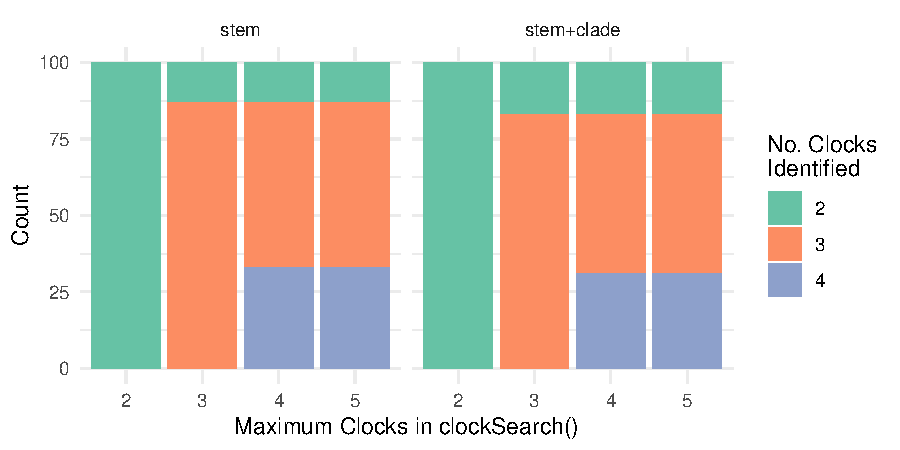
\includegraphics[\linewidth]{figures/inferredClocks.pdf}
\caption{Counts of the number of inferred clocks against the maximum number of clocks allowed by each search. Each plot corresponds to simulated data with either a rate increase along only the stem leading to a clade, or with the rate increase continuing in the clade. The true value is 2 and accuracy decreases as the maximum number of clocks allowed by the clockSearch() algorithm increases.}
\label{fig:simStudy}
\end{figure}



- Include results about speed and accuracy of IC based model selection. Perhaps some RoC cuves?
- Include point about being able to handle trees of $10^5$ tips (phylocanvas anyway). Time this once we get web-workers happening for the BFR.

\section*{Discussion}
- Clockor2 is a flexible framework that is part of the borader shift to web based applications with functionality that can eventually be converted to faster code, such as though bio-rust.
- Future Direction - a pairwise regression that eliminates pseudoreplication in RTT.
- Easier o extend than tempest

\bibliography{clockor2}

\section*{Supplementary Material}
- Derivations for AIC, AICc, and BIC for general strict clock models
\end{document}